% ------------------------------------------------------------------------
% file `arbeitsblatt-example-17-exercise-body.tex'
%
%     exercise of type `example' with id `17'
%
% generated by the `example' environment of the
%   `xsim' package v0.11 (2018/02/12)
% from source `arbeitsblatt' on 2020/10/28 on line 350
% ------------------------------------------------------------------------
In diesem Beispiel beschreiben wir mathematisch den Getränkeautomat.
{\setstretch{1.5}
\begin{enumerate}[(i)]
    \item \(Q =\) \blank[width=0.5\linewidth]{}
    \item \(\Sigma =\) \blank[width=0.5\linewidth]{}
    \item \(q_0 =\) \blank[width=0.5\linewidth]{}
    \item \(F =\) \blank[width=0.5\linewidth]{}
    \item \(\delta:Q \times \Sigma \rightarrow Q \) die Übergansfunktion.
    Wir können alle Werte von \(\delta(q,a)\) für alle \(q \in Q\) und für alle \(a \in \Sigma\) in eine Tabelle schreiben.
        \begin{figure}[H]
\centering
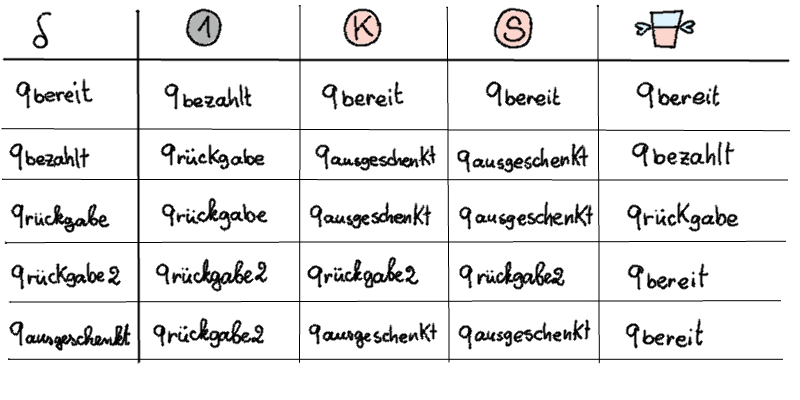
\includegraphics[width=\linewidth]{Pictures/Getraenkeautomat_table_sol.png}
\end{figure}
\end{enumerate}
}
